Midblock crossings are crosswalks that are located on streets in places other than intersections.  They are a safer alternative to pedestrians jaywalking at unmarked points.  Most crosswalks are located at intersections, where traffic lights allow for vehicles to be controlled in order for pedestrians to safely cross the street.  In dense, urban locations with short blocks, this works well.  However, in areas with long stretches of road between intersections, it is not always convenient to have to cross at an intersection.  Many pedestrians will jaywalk across a street at the location where they need to cross it, not necessarily at an intersection.  This can present a hazard to both pedestrians and vehicles, as they could cross the street at any point, and approaching vehicles may not be able to see them.  One study shows that midblock jaywalking was responsible for 26.5\% of all pedestrian accidents \cite{mid1}.

With long blocks, long signals, wide intersections, and high vehicle speeds, crossing at intersections isn’t always easy.  It becomes important to identify points at which it is practical and safe to cross roads.  Without them, pedestrians make their own decisions to cross at random points, creating risk for both themselves and drivers.  By increasing the number of midblock crossings, we hope to decrease the occurrence of jaywalking while improving pedestrian mobility.

\begin{figure}[!htbp]
\centering
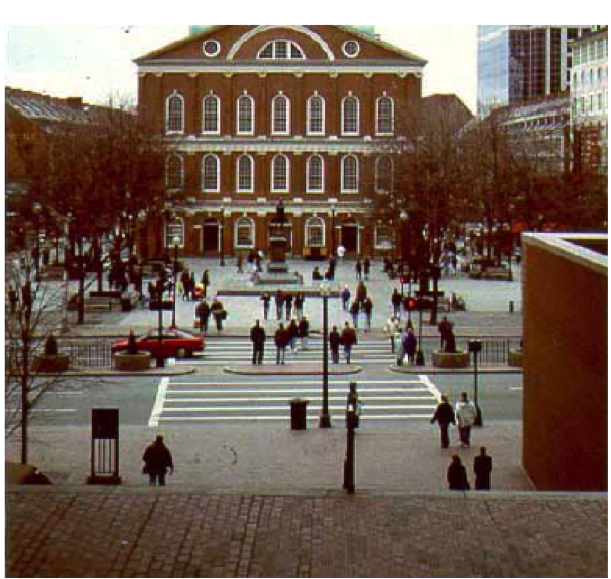
\includegraphics[width=0.5\textwidth]{midblock}
\caption[Midblock Crossing]{Midblock crossings safely connect public places between intersections.}\label{fig:midblock}
\end{figure}

